\documentclass[a4paper,11pt,twoside,openright]{book}
%% For screen reading please replace documentclass with:
%% \documentclass[a4paper,11pt]{report}

\usepackage{graphicx}
\usepackage{algorithmic}
\usepackage{algorithm}
\usepackage{listings}
\usepackage{booktabs}
\usepackage{amsmath}
\usepackage{setspace}
\usepackage{verbatim}
\usepackage[numbers]{natbib}
\usepackage[greek,english,french]{babel}
\usepackage[utf8x]{inputenc}
\usepackage{hyperref}
\usepackage{slantsc}
\usepackage[T1]{fontenc}

%my packages
\usepackage{color}
\usepackage[usenames,dvipsnames]{xcolor}
\usepackage{multirow}
\usepackage{float}
\usepackage{subfig}

\hypersetup{
    bookmarks=true,            % show bookmarks bar?
    unicode=true,              % non-Latin characters in Acrobat’s bookmarks
    pdftoolbar=true,           % show Acrobat’s toolbar?
    pdfmenubar=true,           % show Acrobat’s menu?
    pdffitwindow=true,         % window fit to page when opened
    pdftitle={Master Thesis},  % title
    pdfborder={ 0 0 0 }        % uBorder tin links
}

\long\def\symbolfootnote[#1]#2  
    {\begingroup
    \def\thefootnote{\fnsymbol{footnote}}\footnote[#1]{#2}
    \endgroup}
\renewcommand{\baselinestretch}{1}\small\normalsize
\textwidth=390pt
\oddsidemargin = 50pt
\evensidemargin = 0pt

%% For screen reading please replace odd/even side margin with:
%% \oddsidemargin = 25pt
%% \evensidemargin = 25pt

\newcommand{\worksupportedby}{\symbolfootnote[0]{
Optionally: 
This work was partially supported by {\bf fill in sponsor name}
}}
\newcommand{\thesisdate}{February 2013}

\begin{document}
\lstset{
  language=C++,
  basicstyle=\sffamily,
  columns=flexible,
  numbers=left,
  showstringspaces=false,
  alsoletter={-},
  literate={-}{-}1,
  numbersep=1em,
  xleftmargin=2.5em,
  xrightmargin=1em,
  escapeinside={@}{@},
  commentstyle=\color{gray},
  keywordstyle=\bf\color{blue},
	keywordstyle=[2]\bf\color{blue},
	keywords=[2]{async, future, Futures_Initialize, Futures_Finalize},
	tabsize=2,
}
\begin{titlepage}
\begin{center}

\LARGE \textbf{Implementing Distributed Futures using MPI-2's one-sided commuinication}\\[0.5cm]
\LARGE \textit{Dimitrios Chasapis}\\[0.5cm]

\vfill

\normalsize{
Thesis submitted in partial fulfillment of the requirements for the\\[0.30cm]

\textit{Masters' of Science degree in Computer Science}}\\[0.30cm]

University of Crete\\
School of Sciences and Engineering\\
Computer Science Department\\
Knossou Av., P.O. Box 2208, Heraklion, GR-71409, Greece\\[0.5cm]

\vfill

\Large{Thesis Advisors: Prof. \emph{Joel}, Dr. \emph{Falcou}}\\[0.5cm]

\vfill

\end{center}

\worksupportedby{}
\end{titlepage}

\thispagestyle{empty}

\newcommand{\thesistitle}{Implementing Distributed Futures using MPI-2's one-sided commuinication}
\newcommand{\owner}{Dimitrios Chasapis}
\newcommand{\firstprof}{Joel Falcou}
\newcommand{\secondprof}{Angelos Bilas}
\newcommand{\thirdprof}{Dimitrios S. Nikolopoulos}
\newcommand{\chair}{Yannis Manousakis}

\begin{titlepage}

\begin{center}
\textsc{University of Crete}\\
\textsc{Computer Science Department}\\
\vspace{0.4cm}
\noindent {\textbf{\thesistitle{}}}\\
\vspace{0.4cm}
\noindent Thesis submitted by\\
\textbf{\owner{}}\\
in partial fulfillment of the requirements for the\\
Masters' of Science degree in Computer Science\\
\vspace{0.4cm}
THESIS APPROVAL 

\vspace{0.4cm}

\begin{tabular}{rl}
\\
Author: & \underline{\phantom{123456789012345678901234567890123456789012}}\\
    & \owner{}\\
    \\
    \\
    \\
Committee approvals: & \underline{\phantom{123456789012345678901234567890123456789012}}\\
    & \firstprof{}, Assistant Professor, Thesis Supervisor\\
    & {\small Informatique}\\
    & {\small Universite Paris-Sud XI}\\
    \vspace{0.2cm}
    \\
    \\
& \underline{\phantom{123456789012345678901234567890123456789012}}\\
    & \secondprof{}, Professor\\
    & {\small Computer Science Department}\\
		& {\small University of Crete}\\
    \vspace{0.2cm}
    \\
    \\
& \underline{\phantom{123456789012345678901234567890123456789012}}\\
    & \thirdprof{}, Professor\\
    & {\small School of Electronics,}\\
		& {\small	Electrical Engineering and Computer Science}\\
    & {\small Queen's University of Belfast}
    \vspace{0.2cm}
    \\
    \\
\hspace{1.4ex}Departmental approval: & \underline{\phantom{123456789012345678901234567890123456789012}}\\
    & \chair{}\\
    & {\small  Professor, Director of Graduate Studies}\\
\end{tabular}
\\

\vfill
Paris, \thesisdate{}
\end{center}

\thispagestyle{empty}

\end{titlepage}

\thispagestyle{empty}
\begin{titlepage}
\begin{center}
{\bf\Large Abstract}\\
\end{center}

\paragraph{}
In this work we present a C++11 library implementation of the futures programming model for distributed memory.
Our implementation uses an interface similar to the C++11 standard library's one.  The user can use the 
futures interface to express parallelism and synchronize his code, while the underlying runtime system
schedules the functions the user issues to be run in parallel.  Our runtime currently uses
 the MPI one-sided communication interface, to achieve asynchronous communication.  We evaluate our runtime's
performance and conclude that, in it's current state, it is only suitable for handling coarse grain tasks.
We also share our experience using the MPI one-sided communication interface for implementing a high-performance
runtime. 

\vfill
\end{titlepage}


\thispagestyle{empty}

\selectlanguage{greek}

\begin{titlepage}
\begin{center}

{\bf\Large{Περίληψη}}\\

\end{center}

\indent Στην εργασία αυτή \ldots

\vfill

\end{titlepage}

\selectlanguage{english}

\thispagestyle{empty}
\begin{titlepage}
{\bf\Large Acknowledgements}\\
\paragraph{}
I want to thank my supervisor of this Master Thesis, prof. Joel Falcou for his support and guidance and of-course
for his great sense of humor. It has been a greate experience working with him. I also want to thank my 
other academic supervisors during this Master course, prof. Angelos Bilas and Dimitrios S. Nikolopoulos along with 
Polyvios Pratikakis. They introduced me to parallel computing and languages and their trust and guidance has
inspired and enabled me to complete this work. I also want to thank Antoine Tran Tan for his help and cooperation during the
time I have been working on this Thesis. Finally, I want to express my sincere thanks and love to my family, all my
flatmates, in Greece and France alike, as well as my dearest friends for their support. 

\vfill
\end{titlepage}

\pagenumbering{Roman}
\pagestyle{plain}
\tableofcontents
\listoffigures
\listoftables
\pagenumbering{arabic}
\pagestyle{headings}
\chapter*{Introduction}

\paragraph{}
We present an implementation of the future programming model for distributed memory,
using MPI-2's one-sided communication.  The interface is implemented as a runtime 
library that allows the user to  expose parallelism, by issuing callable functor objects 
asynchronously.  The future object is used like a simple communication channel, where the worker process 
will send through it the return value of the functor object. 
A future object is also used for synchronization. Such an object can be accessed at any time during execution.
The process accessing it will block until the worker process finishes the execution of the functor object, and
transmits the result to the future object.

\paragraph{}
Traditionally futures are implemented using threads in shared memory environments.  
In this work we show that the C++11 standard future interface~\cite{CPP:Threads} can be implemented meaningfully 
for distributed memory machines.  We have chosen to build our system using the MPI-2 one-sided
communication library, so that we can explore and evaluate it's potential to provide a completely asynchronous
communication scheme.  Another reason for using an MPI library is that it is the most commonly message passing
library available on distributed and shared memory machines alike.  
The contributions of this work can sum up to:
\\
\begin{itemize}
	\item Implementation of a unified C++ futures interface for both shared and distributed memory machines, as a runtime system.
	\item Performance Evaluation of the our implementation. 
	\item Evaluation of the MPI-2 one-sided communication interface, for implementing an advanced runtime system.
	\item Exploration of the potential of implementing a runtime on distributed memory using shared memory scheduling techniques.
\end{itemize}

\paragraph{}
Our evaluation shows that the interface implementation is possible, but, performance-wise,  our implementation 
is only able to offer some speedup only when we use coarse grain tasks, due to the high cost of issuing functions 
asynchronously and/or inefficient synchronization schemes. Moreover, MPI-2 one-sided communication interface is 
not as versatile as we would like, especially regarding fine grain synchronization.  

\paragraph{}
The rest of this report is organized as follows:  In chapter \ref{chap:background}, we present the current state
and trends in parallel computing.  We briefly introduce the concept of asynchronous execution models and present
the futures programming model.  At the end of the introduction, we describe MPI's one-sided communication interface.
In chapter \ref{chap:related} we discuss other projects related with our work, and present their approach to
asynchronous communication.  In chapter \ref{chap:implementation} we present in details our system's design and 
implementation.  In chapter \ref{chap:evaluation} we assess our efforts in building the C++11 interface using 
MPI's one-sided communication and use some microbenchmarks and real applications to evaluate the performance
of our runtime system.  Finally, in chapter \ref{chap:conclusion} we give our concluding remarks regarding our
library along with our suggestions for its improvement.    


\chapter{Related Work}
\label{chap:related}

\section{MPI one-sided communication Evaluation}
\paragraph{}
Dinan et al~\cite{Dinan:2012:SGA:2357496.2358660}
have implemented the Global Arrays (GA)\cite{Nieplocha:2006:AAP:1125980.1125985}, a PGAS model, over the one-sided
communication interface of MPI.  In their work they ported GA's low-level ARMCI~\cite{Nieplocha99armci:a} one-sided
communication librari using the MPI API and compared it to ARMCI.  
Although, they succesfully delivered a high-performance runtime, they 
are critical on both interface usability and performance of MPI one-sided interface.  Bonachea in his report
\cite{Bonachea:mpi2} also supports that the MPI one-sided interface is not fit to be used for the implementation 
of PGAS languages.  There are however examples~\cite{A_hydra-mpi:an, Cui:2010:SES:1884643.1884646}
where MPI's one-sided interface has been succesfully used to implement high-performance applications.  

\section{Distributed Futures Implementations}
\paragraph{}
High Performance ParalleX (HPX)~\cite{HPX:TOBE} is a parallel runtime system 
implementation of the ParalleX\cite{Kaiser:2009:PAP:1678991.1679815} 
execution model.  One of ParalleX's many features is the futures synchronization model.
The adopted futures interface is similar to the C++11 standard library one and is available for both shared and distributed
memories.  The model offers additional abstractions to the futures interface, that can be used to describe data-flow relations
and asynchronous computations.
In contrast with our work, it does not use an MPI library for communication, but a different batch system.  

\section{Other asynchronous distributed systems}
\paragraph{}
Other high-performance systems that support Remote Method Invocation (RMI), RSR and RPC share similar specifications
with our runtime system, regarding asynchronous execution.

\paragraph{}
ARMI\cite{Saunders:2003:AAP:966049.781534} is a low-level hybrid (using both threads and message passing) communication library, 
which supports RMI.  In ARMI, objects are shared between threads and processes, but requires manually setting the aggregation
factor in order to have an object's data effectively distributed on processes that do not share a common address space.  On such
case, method calls of the object are done using the library's RMI primitives.  These primitives are implemented on top of MPI and
although they share similar asynchronous charasteristics with our system's implementation, they emulate asynchrony by polling 
at certain time intervals.

\paragraph{}
Tulip\cite{Beckman96tulip:a} is another object-parallel system.  It provides implementations of remote access put/get and RPC 
primitives
over different hardware setups and requires a compiler to create the handlers used in RPC and Active Messages.  In some cases, 
these primitives are implemented using the MPI library and polling for messages, if DMA is not available for communication
between processes.

\paragraph{}
Charm++~\cite{Kale93charm++:a} is an parallel object-oriented extension to the C++ language.  It is based on the 
\emph{Actors}~\cite{conf/icpp/HouckA92} but differentiates sequential and parallel objects.  
It uses a Message driven execution model,
different from the traditional send/receive pairing, where computations begin when a message is received.  The parallel,
work unit in Charm++ is called a \emph{chares} and different \emph{chares} can communicate between themselves.  Instead
of RPC, it uses a futures implementation that provides the same interface for local and remote invocation, in order to have overlapping communication and computation.  This implementation however is not based on MPI or another one-sided 
communication interface.

\paragraph{}
The RSR sheme from Nexus\cite{Foster96thenexus} is similar to the RPC. The user needs to define a handler for the 
RSR that is going to be run remotely, and the data the handler will operate on.  The underlying system will decide
on the mechanism used that the data will be communicated.  Nexus offers a variaty of methods to achieve asynchronous
commonucation in order to remotely execute RSR handlers, depending on available OS and/or hardware.  
We will discuss these different techniques shortly, at the end of this section. 

\paragraph{}
Active-Messages is another communication model, where data that is transfered between processes is paired with 
a handler, which is an action that is performed upon the arrival of data on a process.  This scheme shares some common
asynchronous characteristics with the RPC model. 
AMMPI\cite{Bonachea:ammpi} is an Active-Messages implementation over MPI two-sided communication
interface and LAPI~\cite{Shah:1998:PEL:876880.879642} is a low-level communication library, that offers an interface
similar to Active Messages.  

\paragraph{}
Most of these systems require asynchronous communcation to be effective.  There is a number of known solutions as 
to how to implement such systems in the literature.  The two most commonly used methods are polling for work requests
~\cite{Beckman96tulip:a, Saunders:2003:AAP:966049.781534, Foster96thenexus, vonEicken:1992:AMM:146628.140382} 
and hardware interrupts.
Polling would require a worker process to poll for incoming messages/work at certain
time intervals.   Extra care must be taken to define the polling period, since if polling happens too often, it can
dominate computation, but infrequent polling could render the system unable handle requests in time. 
~\cite{Saunders:2003:AAP:966049.781534, Shah:1998:PEL:876880.879642}.
Alternatively, a hardware interrupt could be sent to notify a process of an incoming message.  This method however,
is avoided because interrupts have to go through the OS, which has a significant cost. 
~\cite{Saunders:2003:AAP:966049.781534, Shah:1998:PEL:876880.879642, Foster96thenexus, vonEicken:1992:AMM:146628.140382}.
The Nexus system ~\cite{Foster96thenexus}, also suggests dedicating threads only for communication.  These threads can 
either probe for pending messages or block (depending on the underlying communication library and OS capabilities).
How responsive this implementation can be depends on the thread implementation and OS (for example if the OS supports
priorities).  A detailed discussion and comparison between using threads for communication versus probing or interrupts
can be found in~\cite{Foster96thenexus}.

\paragraph{}
In our implementation, we use none of these methods, instead we use MPI's one-sided communication interface.  The benefit
of using a one-sided communication interface, lies in the fact that we can have real asynchronous execution.  In contrast 
with polling, the the system can react without any delay (polling period), while it will not suffer from costly interrupts
or the extra overhead and reponse delay of having a thread running, as we discussed above.  However, synchronization in such
a system can become a serious performance problem, as with shared memory models (fences, barries mutexes).





\chapter{Design and Implementation}

	We have implemented the distributed futures using the one-sided mpi library.  

\section{MPI one-sided communication}
maybe should go to the intro

\section{Futures Interface}

\section{Communication}

\section{Memory allocation}

\section{Scheduler}

\chapter{Evaluation}
\label{sect:eval_intro}
	We evaluated our runtime's implementation performance by running some microbenchmark applications and
three small applications (fibonacci, quicksort, LU).  We run all benchmarks on two Intel(R) Xeon(R) 
CPU E5645@2.40GHz with with 6 available cores on each machine, totaling to 12 cores connected through 
a network socket. We have compiled the runtime and application code using g++ version 4.6.3 with 
level 3 optimizations enabled.  For the MPI library we used OpenMPI version 1.4.3.

\section{Microbenchmarks}
\label{sect:microbenchmark}
	Our first microbenchmark is a ping pong application, which is used to measure the time needed to send a 
message from the master to a worker node and the time needed for the worker node to respond back to the master.
Using the future interface, the master simply calls async with a functor that takes a string argument ("ping") 
and returns only a string value ("pong"), without doing any other computations in the functor's body.  We run
the ping pong microbenchmark using the configuration described in~\ref{sect:eval_intro} and the message was 
received by the master in 0.8ms.


	The rest of our microbenchmarks, aim to help us understand better the time needed to issue a job from one
node to another.  To achieve this, we designed one microbenchmark application, where the master node issues
a functor, with only a return statement in his body, which takes a variable number of arguments, each argument
can be either a scalar value or a vector container.  In figure~\ref{fig:issue_time_scalar_vs_containers} we report
the time needed to issue a job that takes a variable number of scalar arguments comparing it with the time needed
to issue a variable number of vector objects of one element.  Although the vector object arguments are more complex
to serialize, we see that the difference in execution time is marginal.  Moreover, we see that the number of arguments
has that need to be transfered, have minimal implact on execution time.  
Figure~\ref{fig:issue_time_different_argnum_same_size} shows the execution time of issuing functor objects with different
vector argument sizes.  In all cases the total number of elements totals to 1200000 (e.g. 1 vector of 1200000 elements or
4 vectors of 300000 elements).   The numbers reported are the median values of 20 runs, and by manual observation 
we can verify that the numbers have been consistent.
As of now, we have no insight as to why having 2 vector objects is more cost efficient
than having only one and the differences cannot be considered "noise". In figure~\ref{fig:job_issue_time_different_argsizes}
we can observe how the size of the arguments can affect execution time.  We see that the size of the arguments (here the 
size of 1 vector object) can exponentially increase execution time.  As expected, the size of the arguments is the factor
that can influence performance the most.

\begin{figure}[!ht]
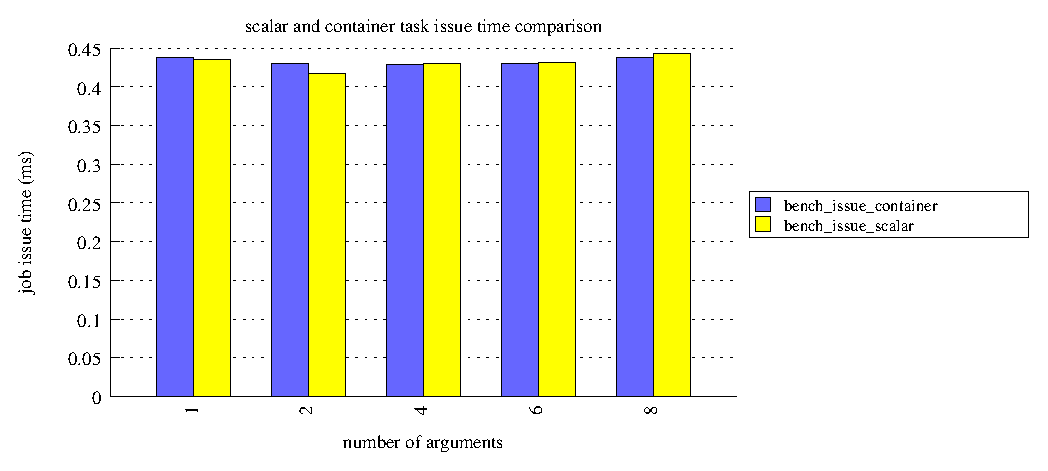
\includegraphics[width=\columnwidth]{figures/job_issue_time_scalar_vs_container_bars}
\caption{Comparison between issuing functors with scalar arguments versus vector objects of size 1}
\label{fig:issue_time_scalar_vs_containers}
\end{figure}

\begin{figure}[!ht]
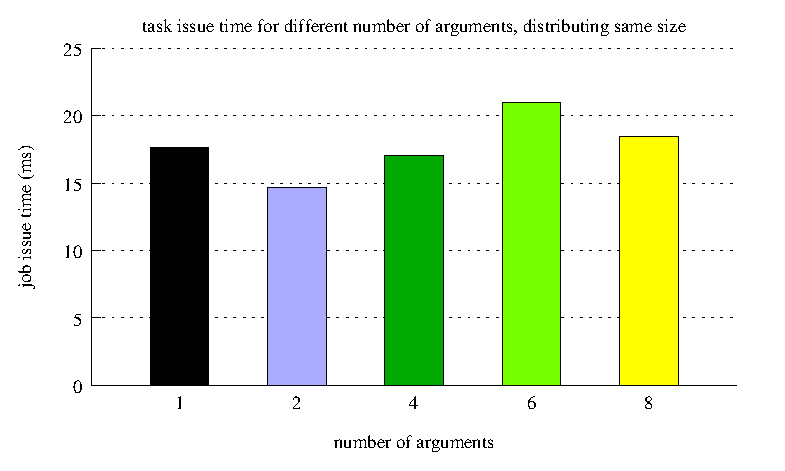
\includegraphics[width=\columnwidth]{figures/job_issue_time_different_argnums_same_size_bars}
\caption{Comparison between issuing functors with different number of vector arguments, but total 
				size of arguments is the same in all cases.}
\label{fig:issue_time_different_argnum_same_size}
\end{figure}

\begin{figure}[!ht]
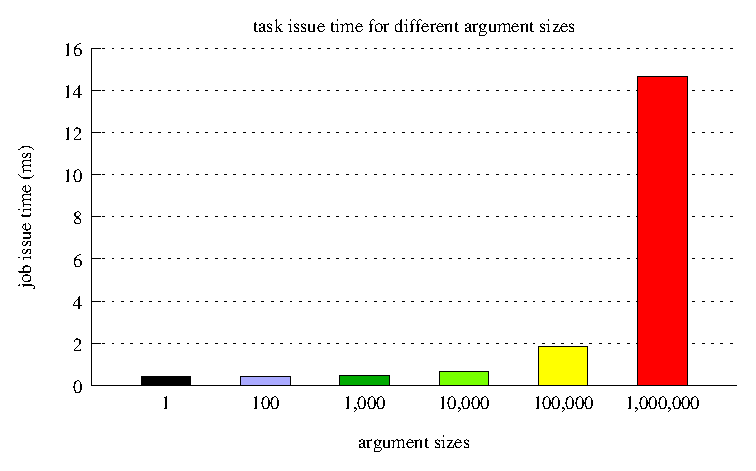
\includegraphics[width=\columnwidth]{figures/job_issue_time_different_argsizes}
\caption{Comparison between issuing functors with 1 vector argument of different sizes}
\label{fig:job_issue_time_different_argsizes}
\end{figure}

\section{Real Application Benchmarking}
\label{sect:real_app}
	In order to evaluate our runtime's performance we have implemented three algorithms using our future's interface.
\\
\\
	\textbf{Fibonacci}:  This is a simple implementation of the fibonacci function.  Figure~\ref{lst:fib} shows 
our implementation.  This recursive version is ideal to demonstrate the ease of use of the future's interface,
but the problem itself is of little interest on a distributed platform, since there is too little work to be 
done on each function.  Nevertheless, we include it in our results.  In our experiments we compute the fibonacci
sequence of 15.
\\
\\
	\textbf{Quicksort}:  Figure~\ref{lst:quicksort} shows our implementation.  The \emph{QsSequantial} 
function itself is a pretty standard
implementation of the common quicksort algorithm.  Parallelization is extracted at the \emph{quicksort} function, where the 
original array is partitioned and asynchrous quicksort functions are called until the \emph{min\_unit} value of elements
is reached, where from that point on the sequential version of the quicksort algorithm is called on each partition.
Notice that for the asynchronous branch of the code, we need to copy each partition in order to send it over the worker 
process and also merge the results of the async functions into the original array.  This additional overhead along with 
the communication overhead makes it necessary to sort small sub arrays sequentially.  For our experiments we sort an 
array of 100,000 doubles. 
\\
\\
	\textbf{Tiled LU}: We have implemented an LU factorization kernel using the Tiled LU algorithm as described in
~\cite{Buttari:2009:CPT:1486274.1486415}.  Figure~\ref(lst:tiledLUseq) shows a simplified version of the tiled
LU algorithm written in C++ style. All arrays are organized in tiles, each tile is a smaller sub array.  Array
\emph{A} is the input array.  In the first step an LU factorization is run on tile \emph{A[k][k]} (\emph{dgetrf} 
function).  The resulting arrays are the lower triangular \emph{L}, the upper triangular \emph{U}, both of which 
are stored in \emph{A[k][k]}, and the transmutation matrix \emph{P[k][k]}.  
The \emph{dgessm} function applies the \emph{L} and 
\emph{U} transformations on all tiles on row k, updating tiles \emph{L[k][k...TOTAL\_TILES]}. \emph{dtstrf}
function performs a block LU factorization on the array formed by coupling the upper triangular part of
\emph{A[k][k]} with \emph{A[k][k]}.
This function returns an upper triangular array, stored in \emph{A[k][k]}, a lower triangular array 
stored in \emph{A[m][k]} and a permutation array P[m][k].  The \emph{dssss} function updates the subarray
formed by tiles \emph{A[k+1...TOTAL\_TILES][k+1...TOTAL\_TILES]} by applying the  transformation computed by \emph{dtstrf}
of the coupled array of the upper triangular part of emph{A[k][n]} and array emph{A[m][n]}.  For the kernels \emph{dgetrf},
\emph{dgessm}, \emph{dtstrf} and \emph{dssssm}, we use the implementation found in the Plasma project
~\cite{1742-6596-180-1-012037} 

	
	Figure~\ref{lst:tiledLUpar} shows a simplified version of our parallel implementation.  The master process 
starts by executing the \emph{dgetrf}  function.  As soon as it completes, we can apply 
the \emph{dgessm} function on the rest of the tiles on row k (k being the step index we are currenlty working on).
Function \emph{dgessm} only requires the L and U factors from \emph{dgetrf} applied on A[k][k], thus we can issue them 
asynchronously, since all dependencies are met
We use here a special array of futures \emph{fA} to hold the return value \emph{dgessm}.   
Next, we apply the blocking LU transformation (\emph{dtstrf}) on the rest of the tiles on column k.  Here, because
each \emph{dtstrf} requires the updated A[k][k] tile from the previous application of \emph{dtstrf}, we cannot issue
them in asynchronously.  Instead, after running a \emph{dtstrf} we immediately issue asynchronous calls to \emph{dssssm}.
This function needs to wait from the \emph{dtstrf} that is applied on the first tile on the row, for the \emph{dgessm}
function that will be applied on the first tile of the column, and from the previous, if any, application of \emph{dgessssm}
on the tile just above the current one, that \emph{dgessssm} is applied.  Because \emph{dssssm} modifies two arrays, we use
a struct to represent the coupling of tile A and the upper triangular array U.  The variable cpldAU, is an array of futures
of that struct type.  The parallelization strategy described, allows us to work on each column asynchronously.  

\begin{figure}[!ht]
\begin{lstlisting}
/* a sequential qs */
void QsSequential(vector<double>& array, const long left, const long right){
    if(left < right){
        const long part = QsPartition(array, left, right);
        QsSequential(array,part + 1,right);
        QsSequential(array,left,part - 1);
    }
}
 
/** A task dispatcher */
class quicksort {
public:
	quicksort() {};
	~quicksort() {};
	vector<double> operator()(vector<double> array, const int deep) {
		const int left = 0;
		const int right = array.size()-1;
    if(left < right){
        if(array.size() > min_unit) {
            const long part = QsPartition(array, left, right);
 						vector<double> subarrA((right)-(part+1)+1), subarrB(part-1-left+1);
						Copy(subarrA, array, part+1, right+1);
						Copy(subarrB, array, left, part);
						quicksort qsort;
						future<vector<double> > res1, res2;
						res1 = async2(subarrA.size(), qsort, subarrA, deep-1);
						res2 = async2(subarrB.size(), qsort, subarrB, deep-1);
            subarrA = res1.get();
            subarrB = res2.get();
						Merge(array, subarrB, subarrA);
        }
        else {
            const long part = QsPartition(array, left, right);
            QsSequential(array,part + 1,right);
            QsSequential(array,left,part - 1);
        }
    }
		return array;
	}
};

\end{lstlisting}
\caption{A quicksort implementation using the distributed futures interface}
\label{lst:quicksort}
\end{figure}


\begin{figure}[!ht]
\begin{lstlisting}
for(int k = 0; k < TOTAL_TILES; k++) {
	dgetrf(A[k][k], P[k][k]);
	for(int n = k+1; n < TOTAL_TILES; n++) {
		dgessm(A[k][n], A[k][k], P[k][k])
	}
  for(int m = k+1; m < TOTAL_TILES; m++) {
		dtstrf(A[k][k], A[m][k] , P[m][k]);
  	for(int n=k+1; n < TOTAL_TILES; n++) {
			dssssm(U[k][n], A[m][n], L[m][k], A[m][k], P[m][k]);
		}
	}
}

\end{lstlisting}
\caption{The tiled LU kernel implementation}
\label{lst:tiledLUseq}
\end{figure}


\begin{figure}[!ht]
\begin{lstlisting}
for(int k = 0; k < TOTAL_TILES; k++) {
	A[k][k] = cpldAU[k][k].get().A;
	dgetrf(A[k][k], P[k][k]);
	for(int n = k+1; n < TOTAL_TILES; n++) {
		A[k][n] = cpldAU[k][n].get().A;
		fA[k][n] = async(dgessm, A[k][n], A[k][k], P[k][k]);
	}
  for(int m = k+1; m < TOTAL_TILES; m++) {
		A[m][k] = cpldAU.get().A;
		dtstrf(A[k][k], A[m][k].get() , P[m][k]);
  	for(int n=k+1; n < TOTAL_TILES; n++) {
			if(m == k+1)
				A[k][n] = fA[k][n].get();
			else
				A[k][n] = cpldAU.get().U;
			A[m][n] = cpldAU.get().A;
			cpldAU[m][n] = async(dssssm, A[k][n], A[m][n], L[m][k], A[m][k], P[m][k]);
		}
	}
}

\end{lstlisting}
\caption{The tiled LU parallel kernel implementation}
\label{lst:tiledLUpar}
\end{figure}

	In figure~\ref{fig:apps_scalability} we report the execution times for running the three applications on the
machine setup we described in section~\ref{sect:eval_intro}.  We measure only the algorithm and no initialization
and finalization times of the runtime system, etc.
We observe that we do not manage to get any speedup on 
any application, on the contrary we get a slowdown (figure~\ref{fig:apps_speedup}).
There is some improvement as we increase the cores for 
the fibonacci and quicksort applications, but in no case we manage to even match the sequential problem.  In 
figure~\ref{fig:apps_breakdowns_6cores} 
we show the breakdowns for the master application and the slaves, for running the applications on 6 cores.
\emph{Job issue time} is the time needed to send a \emph{job} from one process to another. This time includes
time spend in the scheduler, to find the next worker and time spend on serialization of the \emph{job} object
and sending it to the worker.  \emph{Job execution time} is the time spent on running the actual code of the
\emph{job} that was issued via an async call.  \emph{User code time} is the time the master process spends
running code that is not related with the runtime.  \emph{Idle time} is time spend waiting to retrieve a future 
value and for the workers, it's also time spent waiting for a \emph{job} to become available in their stacks.
\emph{Rest of time} is the rest of the overhead that is imposed by the runtime.  This time can be for example 
the time needed to send the return value of the asynchronous execution of a \emph{job} by a worker.  In all 
applications we see that the either \emph{job issue time} or \emph{rest of time} are the greatest sources of 
overhead, while a fair amount of time is also spent on \emph{idle time}.  These overhead times are too great
compared to the actual work done by any of the processes, so small problems and kernels are not fit to be 
run on our runtime system, as the current implementation stands.  At this stage it is unclear whether the issue
is the MPI library or the implementation.  We will further investigate the current issues.  Moreover, figure
~\ref{fig:app_breakdowns_w_init} shows the same breakdowns with figure~\ref{fig:app_breakdowns_6cores}, with 
the addition of initialization and finalization times.  The initialization and finalization include the 
creation and finalization of the communication module (in our experiments that's MPI), creation and destruction
of the shared memory (MPI Windows) and scheduler.  The initialization time is constant on all applications, since
it mainly depends on the number of processes, while the finalization time is negligible. 

\begin{figure}[!ht]
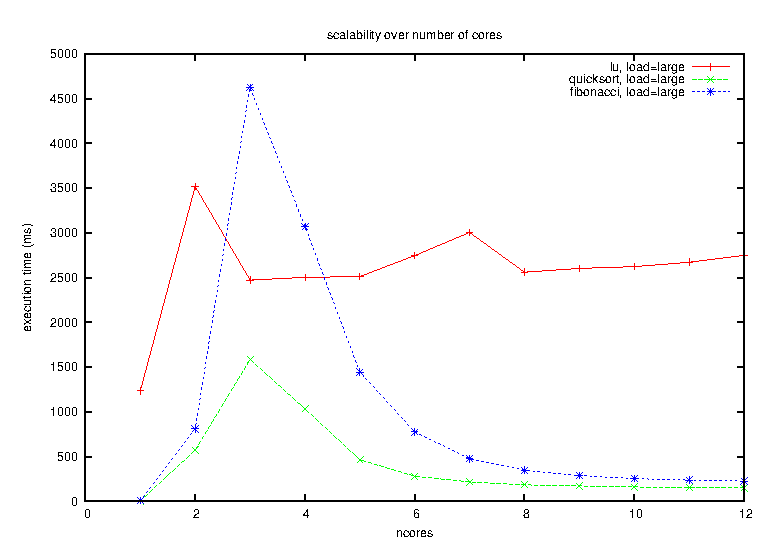
\includegraphics[width=\columnwidth]{figures/apps_scalability}
\caption{Scalability graph for fibonacci, quicksort and LU}
\label{fig:apps_scalability}
\end{figure}

\begin{figure}[!ht]
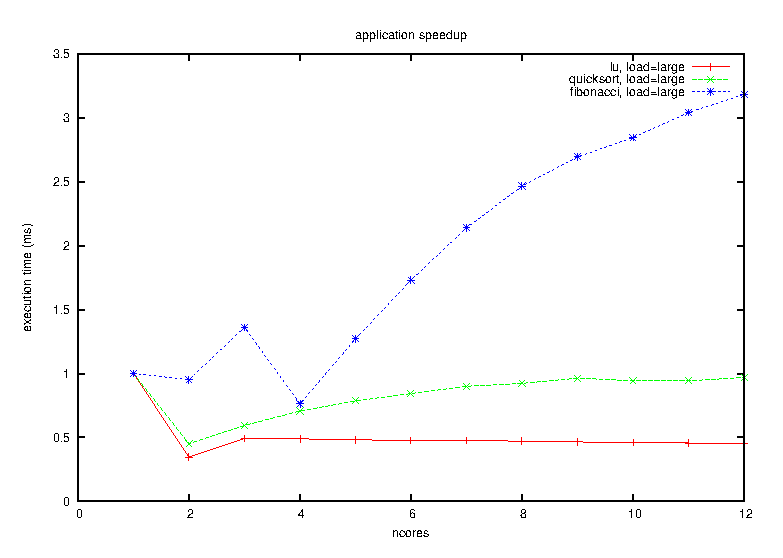
\includegraphics[width=\columnwidth]{figures/apps_speedup}
\caption{Speedup graph for fibonacci, quicksort and LU}
\label{fig:apps_speedup}
\end{figure}

\begin{figure}[!ht]
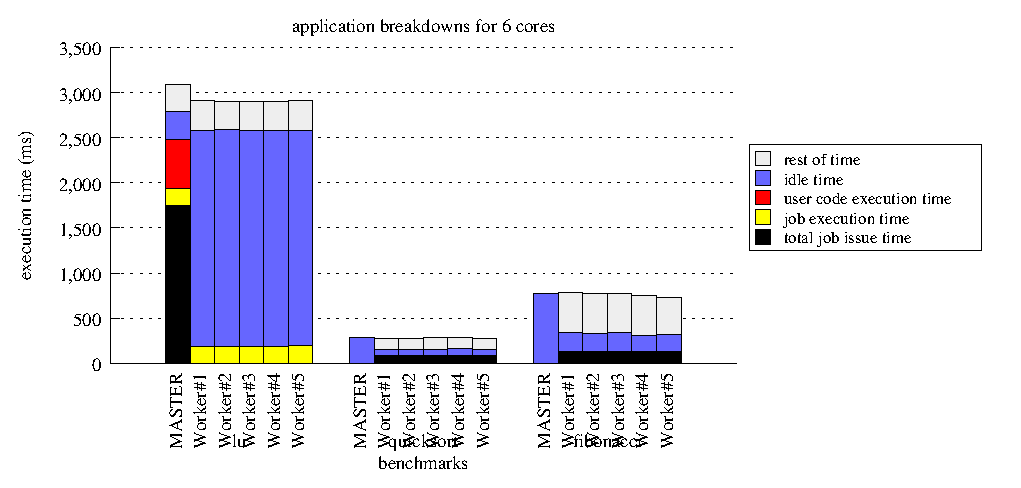
\includegraphics[width=\columnwidth]{figures/app_breakdowns_6cores}
\caption{Breakdowns of master and worker execution time graph for fibonacci, quicksort and LU}
\label{fig:app_breakdowns_6cores}
\end{figure}

\begin{figure}[!ht]
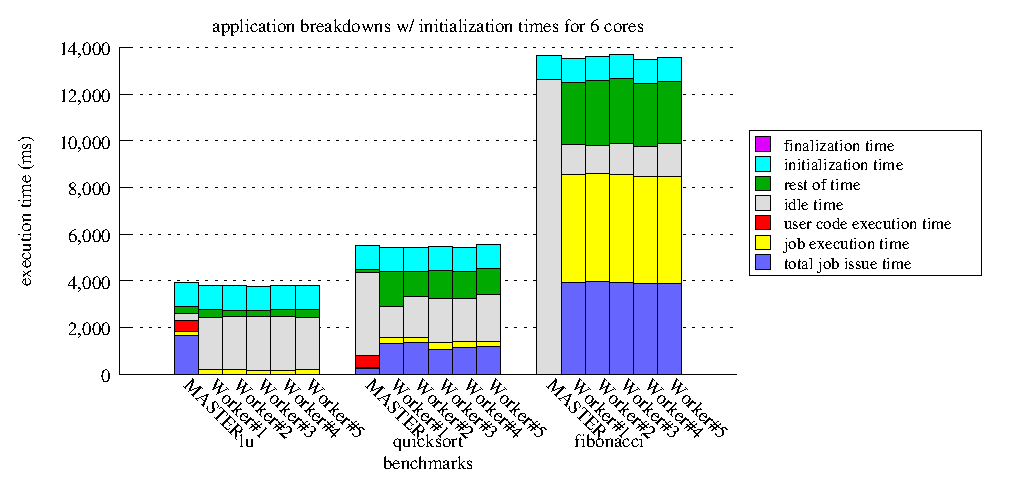
\includegraphics[width=\columnwidth]{figures/app_breakdowns_w_init}
\caption{Breakdowns of master and worker execution time graph for fibonacci, quicksort and LU, with initialization
and finalization times}
\label{fig:app_breakdowns_w_init}
\end{figure}




\chapter{Conclusions and Future Work}
In this work we presented an implementation of the futures programming model as a C++ library,
for distributed memory machines.  We implemented our system using the MPI one-sided communication
library for communication and we adopted shared memory scheduling techniques to implement 
our scheduler, making use again of the MPI one-sided interface.  Our evaluation of the system shows
that the current implementation suffers from significant overheads, especially when issuing asynchronous
\emph{jobs} on processes. In order to be usable, the user must issue coarse grain \emph{jobs}.  At this
point, we are inconclusive whether the large overhead can be attributed to the MPI library or to other
implementation issues in our runtime system (e.g. scheduling policies, mutex implementation).  We suspect
however, that busy waiting, the technique we use to check for future availability, 
even on local variable that are shared through MPI windows can be costly (acquiring locks on an "epoch" for example).


At this point, from our experience with the MPI one-sided communication interface, we believe that there exist
some fundamental limitations in its design. These are:
\\
\begin{enumerate}
	\item MPI\_Window creation is a collective operation over a group of MPI processes.  In order to dynamically
				allocate data and share through a window, all processes must synchronize, calling the MPI\_Window\_create
				routine.  For our asynchronous system this is a serious limitation, especially when we only want to create
				windows between only two processes at a time.  The only solution to this problem would be to create a priori
				all possible groups for all pairs of processes, which can be costly.  Instead, we were forced to preallocate
				a buffer for each process, that is shared through a window.
	
	\item The \emph{active mode} "epoch" definition scheme, requires both processes to take part in the communication,
				which we believe to be counter intuitive for an one-sided communication interface. What's more, we find that
				it is unusable in our asynchronous communication system.

	\item The locking schematics of the \emph{passive mode} "epoch" definition scheme, do not define well what happens
				when a window is concurrently accessed, which can cause erroneous results.  This forced us to implement our
				own mutexes to synchronize data accesses on the same window.  Moreover, acquiring an exclusive lock on a 
				window will block other processes from accessing it, even if they access different, non-overlapping addresses
				in that window.  The later constraint, limits fine grain locking.  In our system, this is a very common
				scenario, where processes, different asynchronous \emph{jobs}, need to write to different parts of the same
		 		window of the process owning the associated futures.   
\\
\end{enumerate}

In the future we plan to further investigate the cause of our systems high overhead.  If our suspicions are correct
and the cause of the overhead is our scheduling scheme, we will try different approaches than using the MPI one-sided
communication in order to achieve better performance.  Our focus will be to deliver a high performance runtime system.
We also plan to add important features to the runtime, such as the ability to serialize and send futures to other 
processes.  This will be very useful in applications like our Tiled LU, where the master issues all the async \emph{jobs},
but instead each process will wait for it's futures to be available. This will allow finer grain synchronization and
the master will not become a bottleneck.


\bibliographystyle{IEEEtran}
\bibliography{references}

\end{document}
